\chapter[Modeling of H-SCC]{Modeling of Hybrid Switched Capacitor Converters}

Switch capacitor converters are circuits composed by a large number of switches and capacitors, and require accurate models to properly design them. SCCs have the peculiarity to be lossy by nature due to the non adiabatic energy transfer between capacitors, phenomenon not present in the inductor based converters. Generally, modeling of SCCs focuses just on  the description of the loss mechanisms associated to conduction and capacitor charge transfer, neglecting other sources of loss such as driving and switching loss. These loss mechanisms are proportional to the output current, thus are normally modeled with resistor in the well known output impedance model.

This chapter presents a new methodology to model a SCC when any of the nodes in the converter are loaded. The proposed methodology also include the effects of PWM control, thus accurately predicting the equivalent internal impedance and the converter conversion ratio.

The chapter is divided in two sections, the first section is devoted to the study and model a SCC when loaded from a \emph{pwm}-node, reviewing and extending the charge flow analysis~\cite{95Makowski,Seeman:EECS-2009-78} to include two new aspects that arise with the proposed hybrid converter. First, any of the nodes of the converter are considered as possible outputs that can be loaded. Second, the analysis includes the effects of duty cycle (PWM) in any of the operation regimes of the converter, and this alters the conversion ratio and the internal equivalent impedance. The previous models are discussed, and the limiting are factors identifying. Subsequently the charge flow analysis is reformulated using a new approach based on current-loaded outputs that leads a better accuracy and covers the analysis of both SCC and H-SCC. The new model is compared to circuit simulations and experimental data.

The second section is devoted to the study of multiple loaded H-SCC. Based on the well-known output impedance model, a new circuit representation for converters with multiple current-loaded outputs is presented. The related characterization methodology is developed to determine the parameters of said new model based on the current-loaded analysis presented in the first section. The resulting model is validated against simulation and experimental data.


\section{Single Output Converters}
Switched Capacitor Converters has been always treated as a two-port converter with single input and a single output as shown in Fig.\ref{fig:two_port}. The input port is connected to a voltage source and the output port feeds the load. The SCC provides between input, $v_i$, and output, $v_o$, a voltage conversion, $m$,  that  steps up, steps down or/and inverts the polarity of the input voltage. Up to present all the circuit theory devoted SCCs is valid only for the two-port configuration, therefore this section is dedicated to revisit the classical concepts of single output SCC and to introduce new ones that enable to study the H-SCC.

\begin{figure}[!h]
\centering
\ctikzset { bipoles/length=1cm}
\begin{circuitikz}[american voltages,scale=0.65]
\draw
    (1,0) to[short,o-]
    (0,0) to[V = $V_{supply}$]
    (0,3) to[short,-o]
    (1,3) ;

\draw
    (2,3) --
    (2.5,3)

    (2,0) --
    (2.5,0)

    node[ocirc]  (IC)  at (2,0) {}
    node[ocirc]  (I) at (2,3) {}
    (I) to[open,v=$v_{i}$] (IC);


\draw [thick]
    (2.5,-0.5) --
    (2.5,3.5)  --
    (5.5,3.5)  --
    (5.5,-0.5) --
    (2.5,-0.5);

\draw (4,2)node[anchor=north]{$\frac{v_o}{v_{i}}=m$} ;
\draw
    (5.5,3) -- (6,3)
    (5.5,0) -- (6,0)
    node[ocirc]  (O)  at (6,3) {}
    node[ocirc]  (OC) at (6,0) {}
    (O) to[open,v^<=$v_{o}$] (OC);

\draw
    (7,0) to[short,o-]
    (8,0) to[ R= $Load$,mirror]
    (8,3) to[short,-o]
    (7,3) ;
\end{circuitikz}
\caption{General two port configuration of a Switched Capacitor Converter. }
\label{fig:two_port}
\end{figure}

\subsection{The Output Impedance Model}
The behavior of SSCs is modeled with the well-known output impedance model~\cite{2000Oota,2012Peter} that is composed of a controlled voltage source and equivalent resistance $r_{scc}$, as shown in figure~\ref{fig:scc_model_oi}.The output voltage provided by the converter under no-load conditions is defined as \emph{target voltage} ($v_{trg}$). It is modeled with the controlled voltage source, being the value of voltage supply $v_{src}$ multiplied by the conversion ratio $m$, thus
\begin{equation}
v_{trg} =  m \cdot v_{src} .
\label{eq:vtrg}
\end{equation}

When loaded, the voltage droop across $r_{scc}$ accounts for the loss produced in the converter: capacitor charge transfer loss and conduction loss. In fact, the loss are proportional to the output current $i_o$, that is why they are represented with a resistor. Hence the output voltage of the converter can be obtained as
\begin{equation}
v_{out} =  m \cdot v_{src} - i_o \cdot r_{scc} .
\label{eq:vout_scc}
\end{equation}

\begin{figure}[!h]
\centering
\ctikzset { bipoles/length=1cm}
\begin{circuitikz}[american voltages, scale=0.65]
\draw
    (-0.5,0) to[V = $ m \cdot v_{src}  $]
    (-0.50,3) -- (0,3) to[R,l=$r_{scc}$,-o]  (3,3)
    (3.5,3) to[short,o-,i=$i_o$]
    (4.25,3)   to[R,l=$r_o$]
    (4.25,0) to[short,-o] (3.5,0)
    (3,0) to[short,o-] (-0.5,0)
    (0,3) to[open,v^=$v_{trg}$] (0,0)
    (3.5,3) to[open,v=$v_{out}$] (3.5,0);

\end{circuitikz}
\caption{Output impedance model of a switched capacitor converter.}
\label{fig:scc_model_oi}
\end{figure}

Up to day, there are two different methodologies to infer the model parameters: $m$ and $r_scc$. On the one hand, S. Ben-Yaakov  ~\cite{2009Ben-Yaakov,2012Ben-Yaakov,2013Evzelman} has claimed a generalized methodology based on the analytical solution of each of the different transient circuits of the converter, reducing all of them to a single transient solution. The methodology achieves a high accuracy, but yields to a set of none linear equations and high complexity for the analysis of advanced architectures.

On the other hand,  M. Makowski and D. Maksimovic~\cite{95Makowski} presented a methodology based on the analysis of the charge flow between capacitors in steady-state. The methodology is simple to apply and yields with a set of linear expressions, being them easy to operate for further analysis of the converters. Based on the charge flow analysis, M.Seeman~\cite{Seeman:EECS-2009-78} developed different metrics allowing to compare performances between capacitive and inductive converters.  Although both methodologies are valid in the modeling of SCCs, none of them has been used to model the effects of a loaded \emph{pwm}-node, which is fundamental to study the H-SCC.  Nevertheless the charge flow analysis has a more clean and simplified way of describing the loss mechanism, based on the hypothesis that a SCC in steady-state has to have null charge balance in all the capacitors. That is why this methodology has been chosen in to model the H-SCC, although few modeling hypothesis have been reviewed and modified according with operation of the new \emph{hybrid} converter.

\subsection{Revising the charge flow analysis}
The charge flow analysis method is based on charge conservation in the capacitors during a switching period when the converter is in steady state~\cite{95Makowski}. Based on the charge flow of the capacitors, the converter is studied in two well-defined operating regimes: the Slow Switching Limit (SSL) and the Fast Switching Limit (FSL). In SSL, the converter operates at a frequency much lower than the time constant of the converter, thereby allowing the full charge and discharge of the capacitors. The losses are then dominated by the charge transfer between capacitors. In FSL, the converter operates with a switching frequency much higher than the time constant of the converter, limiting the charge and discharge transient times of the capacitors. Conduction losses due to the parasitic resistive elements ($r_{on}$, $c_{esr}$) therefore dominate.\\

The charge flow method~\cite{95Makowski} makes some assumptions in order to model the SCC. First, the load is modeled as an ideal voltage source since it is normally connected to the \emph{dc}-output in parallel with a large capacitor. This ignores the contribution of the output capacitor to the equivalent resistance of the model. Second, the model only considers the \emph{dc}-output as the single load point of the converter, imposing a unique output to the converter. Third, the phase time ratio is not included in the computation of the capacitor charge flow. Consequently, the modulation of the switching period is assumed to have no influence on the amount of charge flowing in the capacitors. These simplifications reduce the usability of the model to the specific application of dc-to-dc conversion, and at the same time limit the flexibility to model different concepts of the SCC, such as the aforementioned hybrid concept. In order to overcome these limitations, the presented methodology makes two different assumptions: First, any of the converter nodes can be loaded. Second, the load is assumed to be a constant current source with a value equal to the average load current.\\


\subsection{Re-formulating the charge flow analysis}

The SSL impedance encompasses the losses produced in the charge transfer from capacitor to capacitor and from voltage supply to capacitor; therefore, for this analysis none of the parasitic resistances are taken into account. As mentioned before, the classical approach to study SCCs is to assume an infinitely large output capacitance connected to a \emph{dc}-node, an approach that has two limitations:
\begin{enumerate}
   \item Produces inaccuracies when the output capacitor is comparable in value to the flying capacitors.
   \item Cannot be used for a converter with a load connected to one of the internal nodes.
\end{enumerate}


\begin{figure}[!h]
\centering
\ctikzset { bipoles/length=1cm}
\begin{subfigure}[t]{.4\textwidth}
    %\centering
    \raggedright
    \begin{circuitikz} [american,scale=0.65]
    \draw
        (0,0) to[V=$v_{src}$] (0,3)
        (3,3) to[pC,l=$c_1$] (0,3)
        (3,0) to[pC,l=$c_2$] (3,3) -- (6,3)
        (6,0) to[pC,l=$c_3$] (6,3) --
        (8,3) to[I,l=$i_o$] (8,0) -- (0,0);
    \begin{scope}[>=latex,thick,text=black]
        \draw [->,rounded corners=7pt,dashed]
            (0.4,2.4) -- (2.4,2.4) -- (2.4,0.4);
        \draw [->,rounded corners=7pt,dashed]
            (3.6,0.5) |- (5.4,2.7) -- (5.4,0.4);
        \draw [->,rounded corners=7pt]
             (6.3,2) |- (8,3.3);
        \draw [>=latex,text=black,dashed]
          (0,4)  -- (0.9,4) node[anchor=west]{Redistributed charge};
        \draw [>=latex,text=black]
          (0,4.5)  -- (0.9,4.5) node[anchor=west]{Pumped charge};
    \end{scope}
    \end{circuitikz}
    \caption{}
\end{subfigure}
\hfill
\hfill
\begin{subfigure}[t]{.4\textwidth}
    %\centering
    \raggedleft
    \begin{circuitikz} [american,scale=0.65]
    \draw
        (1,0) to[V=$v_{src}$] (1,3)
        (6,3) to[pC,l=$c_2$] (3,3)
        (3,0) to[pC,l=$c_1$] (3,3)
        (6,0) to[pC,l=$c_3$] (6,3) --
        (8,3) to[I,l=$i_o$] (8,0) -- (1,0);
    \begin{scope}[>=latex,thick,text=black]
        \draw [->,rounded corners=7pt,dashed]
            (3.6,0.5) |- (5.4,2.4) -- (5.4,0.4);
        \draw [->,rounded corners=7pt]
            (6.3,2) |- (8,3.3);% -- (8.6,0.4);

    \end{scope}
    \end{circuitikz}
    \caption{}
\end{subfigure}
\caption{Charge flows in a Dickson 3:1 converter when loaded at a \emph{dc}-node with a large capacitor during the two switching phases. The solid line marks the pumped charge to the load and the dashed lines the possible paths of the redistributed charge.}
\label{fig:charge_flow_I}
\end{figure}

In the original charge flow analysis of the SSL impedance~\cite{95Makowski}, it is assumed that all of the pumped charge to the load is only supplied by a \emph{dc}-capacitor without any \emph{pumping} contribution from the flying capacitors, as shown in figure~\ref{fig:charge_flow_I}.  However, for a finite value of the output capacitor, or for converters loaded from an internal node, all of the capacitors contribute to pumping charge to the load~\cite{2013Breussegem:c_out}, as shown in figure~\ref{fig:charge_flow_II}. The original analysis omitted the \emph{pumped} charge contribution of the flying capacitors, thereby overestimating the \emph{redistributed} charge, resulting in an overestimation of the SSL impedance.

\begin{figure}[!h]
\centering
\ctikzset { bipoles/length=1cm}
\begin{subfigure}[t]{.4\textwidth}
    %\centering
    \raggedright
    \begin{circuitikz} [american,scale=0.65]
    \draw
        (0,0) to[V=$v_{src}$] (0,3)
        (3,3) to[pC,l=$c_1$] (0,3)
        (3,0) to[pC,l=$c_2$] (3,3) -- (6,3)
        (6,0) to[pC,l=$c_3$] (6,3) --
        (8,3) to[I,l=$i_o$] (8,0) -- (0,0);
    \begin{scope}[>=latex,thick,text=black]
        \draw [->,rounded corners=7pt,dashed]
            (0.4,2.4) -- (2.4,2.4) -- (2.4,0.4);
        \draw [->,rounded corners=7pt,dashed]
            (3.6,0.5) |- (5.4,2.7) -- (5.4,0.4);

        \draw [->,rounded corners=7pt]
            (2,3.3) -- (7,3.3)
            (2.7,2) |- (7.5,3.3)
            (6.3,2) |- (8,3.3);
        \draw [>=latex,text=black,dashed]
          (0,4)  -- (0.9,4) node[anchor=west]{Redistributed charge};
        \draw [>=latex,text=black]
          (0,4.5)  -- (0.9,4.5) node[anchor=west]{Pumped charge};
    \end{scope}


    \end{circuitikz}
    \caption{}
\end{subfigure}
\hfill
\hfill
\begin{subfigure}[t]{.4\textwidth}
    %\centering
    \raggedleft
    \begin{circuitikz} [american,scale=0.65]
    \draw
        (1,0) to[V=$v_{src}$] (1,3)
        (6,3) --  (3,3)
        (3,0) to[pC,l=$c_1$] (3,3)
        (6,0)-- (6,0.25) to[pC,l=$c_3$] (6,1.5) to[pC,l=$c_2$] (6,2.75) |-
        (8,3) to[I,l=$i_o$] (8,0) -- (1,0);
    \begin{scope}[>=latex,thick,text=black]
        \draw [->,rounded corners=7pt,dashed]
            (3.6,0.5) |- (5.4,2.7) -- (5.4,0.4);
        \draw [->,rounded corners=7pt]
             (2.7,2) |- (7.5,3.3)
             (6.3,2.5) |- (8,3.3);% -- (8.6,0.4);
    \end{scope}
    \end{circuitikz}
    \caption{}
\end{subfigure}
\caption{Charge flows in a Dickson 3:1 converter when loaded at one of the \emph{pwm}-nodes during the two switching phases. The \emph{solid} lines marks the pumped charge paths to the load and the \emph{dashed} lines the possible paths of the redistributed charge.}
\label{fig:charge_flow_II}
\end{figure}

In order to overcome the restrictions of the original charge flow methodology, the proposed methodology models the load as a current sink instead of a voltage sink. This slight modification has a relevant change in the modeling of the converter, adding three important aspects to the modeling:
\begin{enumerate}
  \item Connect the load to any of the nodes of the converter, since it does not fix any voltage at the connected node.

  \item Include the \emph{dc}-capacitors in the analysis, since the voltage across the sink is given by the capacitor and not longer by the previous used voltage sink.

  \item Estimate the delivered charge to the load for each of the circuit modes of the converter, since the current sink has a value of the averaged output current.
\end{enumerate}

\subsubsection[SSL]{Slow Switching Limit}

A charge multiplier vector $\mathbf{a}$ is obtained for all of the operation modes, also known as phases, of the converter. The charge multiplier vector corresponds to the charge flowing in every individual capacitor or source, normalized with respect to the total output charge $q_{out}$, as described in~\cite{95Makowski,Seeman:EECS-2009-78}. Owing to the fact that load current $i_o$ is assumed constant, the output charge of the $j$-phase can be expressed as the ratio of the phase duration $D^j$ to the total switching period $T_{sw}$, and its contribution to the total output charge $q_{out}$ is
\begin{equation}
    q^j_{out} = i_{o} T_{sw} D^j = D^j q_{out} .
\label{eq:qout}
\end{equation}

Each charge flow element $ a(D^j)_i^j$  is a function of the phase duration $D^j$ and corresponds to the total net charge circulating in the $i$-th capacitor $c_i$ during the $j$-th phase, and can be used to compute the $net$ voltage $v_n$ variation at the end of the $j$-th phase period:
\begin{equation}
\Delta {v_n}^j_i  = \frac{a_i ^j }{c_i} q_{out} .
\label{eq:net_voltage}
\end{equation}

The current flowing through the $i$-th capacitor can be assumed to be constant, since the load has been modeled as a constant current skin. Hence the current in the $i$-th capacitor will a

 Due to the approximation of constant load current, it can be assumed that in the $i$-th capacitor the charge to the load is pumped by a constant current $i_i$.


Hence the pumped voltage $v_p$ variation during the $j$-th phase of the total switching period $T_{sw}$ can be simply computed as
\begin{equation}
\Delta {v_p}^j_i  = \frac{i_i^j}{c_i} T_{sw} D^j = \frac{a_i ^j }{c_i} q_{out} .
\label{eq:pumped_voltage}
\end{equation}


\begin{figure}[!h]
\centering
% This file was created by matlab2tikz.
%
%The latest updates can be retrieved from
%  http://www.mathworks.com/matlabcentral/fileexchange/22022-matlab2tikz-matlab2tikz
%where you can also make suggestions and rate matlab2tikz.
%

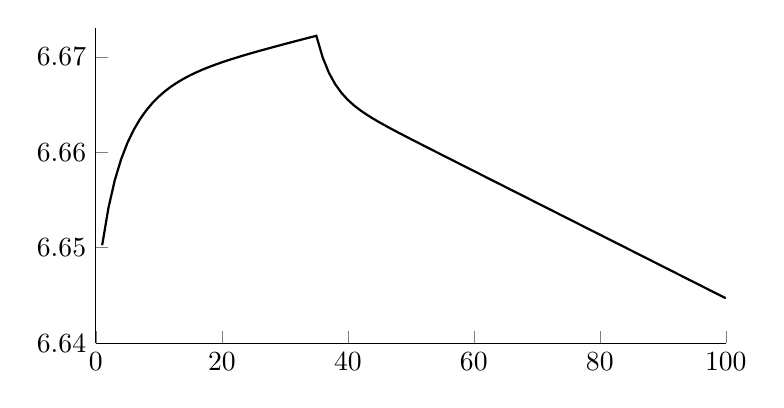
\begin{tikzpicture}

\begin{axis}[%
width=8cm,
height=4cm,
at={(1.532in,0.729in)},
scale only axis,
xmin=0,
xmax=100,
ymin=6.64,
ymax=6.673,
axis background/.style={fill=white},
axis x line*=bottom,
axis y line*=none
]
\addplot [thick,solid,forget plot]
  table[row sep=crcr]{%
1	6.65026844706453\\
2	6.6541906445053\\
3	6.65706994984393\\
4	6.65925863469407\\
5	6.66097190927411\\
6	6.66234478933293\\
7	6.66346632700282\\
8	6.66439739781252\\
9	6.66517963724446\\
10	6.66584465605996\\
11	6.66641623072511\\
12	6.66691268208139\\
13	6.66734838569269\\
14	6.6677347707153\\
15	6.66808100843884\\
16	6.66839450570606\\
17	6.66868127063699\\
18	6.66894619123669\\
19	6.66919325215929\\
20	6.66942570599671\\
21	6.66964621014256\\
22	6.66985693700001\\
23	6.67005966319872\\
24	6.67025584208054\\
25	6.67044666273543\\
26	6.67063309816195\\
27	6.67081594459879\\
28	6.67099585366935\\
29	6.67117335866543\\
30	6.67134889604556\\
31	6.67152282302303\\
32	6.67169543195692\\
33	6.67186696212833\\
34	6.67203760937764\\
35	6.67220753399144\\
36	6.66994898046201\\
37	6.66832576586377\\
38	6.66712775868683\\
39	6.66621535139474\\
40	6.66549387715858\\
41	6.66490036899855\\
42	6.66439286198158\\
43	6.6639431930172\\
44	6.66353165635979\\
45	6.66314608322637\\
46	6.6627778080521\\
47	6.66242109657901\\
48	6.66207215837762\\
49	6.6617284123912\\
50	6.66138813136178\\
51	6.66105016231045\\
52	6.66071373588587\\
53	6.66037833874885\\
54	6.66004362838354\\
55	6.659709376253\\
56	6.65937542987049\\
57	6.65904168749229\\
58	6.6587080812319\\
59	6.65837456579342\\
60	6.65804111199682\\
61	6.65770769693504\\
62	6.65737430934867\\
63	6.65704093984341\\
64	6.65670758237776\\
65	6.65637423294288\\
66	6.65604088886614\\
67	6.65570754836448\\
68	6.65537421024822\\
69	6.65504087372358\\
70	6.65470753826091\\
71	6.65437420350682\\
72	6.65404086922551\\
73	6.65370753525966\\
74	6.6533742015043\\
75	6.65304086788937\\
76	6.65270753436815\\
77	6.65237420090945\\
78	6.65204086749247\\
79	6.6517075341038\\
80	6.65137420073293\\
81	6.65104086737468\\
82	6.65070753402473\\
83	6.65037420068031\\
84	6.65004086733958\\
85	6.64970753400131\\
86	6.64937420066469\\
87	6.64904086732916\\
88	6.64870753399436\\
89	6.64837420066005\\
90	6.64804086732606\\
91	6.64770753399229\\
92	6.64737420065867\\
93	6.64704086732514\\
94	6.64670753399168\\
95	6.64637420065826\\
96	6.64604086732487\\
97	6.6457075339915\\
98	6.64537420065814\\
99	6.64504086732479\\
100	6.64470753399144\\
};
\end{axis}
\end{tikzpicture}%
\caption{The two possible voltage waveforms that show the capacitors in a SCC. Ripples are associated with the charge flow mechanisms: top) unipolar capacitor discharge (DC capacitor); bottom) bipolar capacitor discharge (flying capacitor).}
\label{fig:charge_flow_I}
\end{figure}


\subsubsection[FSL Switch Charge Flow]{Fast Switching Limit: Re-defining the Switch Charge Flow Vectors}

\subsection{Load Model: Voltage Sink versus Current Sink}
\subsection{Sensitivity of the inductor current ripple}

\section{Multiple Output Converters}
\subsection{The Output Trans-Resistance Model}
\subsection{Obtaining the Trans-Resistance parameters with the charge flow analysis }



\chapter[Optimization and Design]{Optimization and Design of Hybrid-Switched Capacitor Converters}
\section{Introduction}
\section{Study in the correlation of the design parameters and the Output Impedance}
\section{Encapsulating the Switches and Capacitors area breakdown in an optimization procedure}
\section{Insights towards a complete optimization}

\chapter[Dynamic Study]{Dynamic Study of Hybrid-Switched Capacitor Converters}
\section{Small Signal Analysis}


\clearpage
\bibliographystyle{plainnat}
\bibliography{references} 